\documentclass{standalone}
\usepackage{pgfplots}
\begin{document}	
	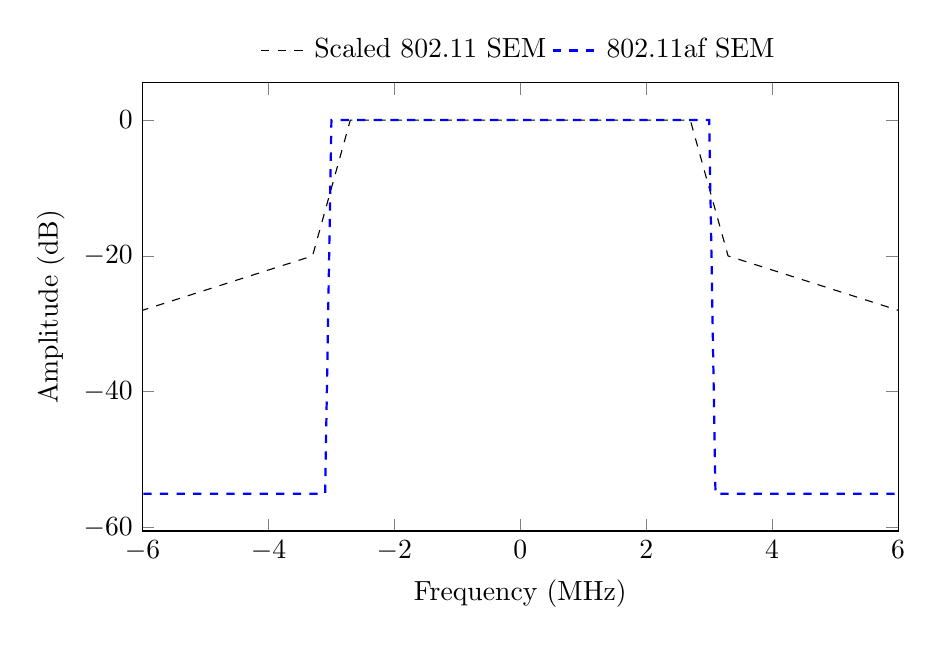
\begin{tikzpicture}
	\begin{axis}[ xlabel=Frequency (MHz), ylabel= Amplitude (dB), legend columns=4,	legend style={at={(0.5,1.02, ultra thick)}, anchor=south, cells={anchor=west}, draw=none}, xmin=-6, xmax=6, x post scale=1.4]
		%\addplot+[style={dashed, color=black}, every mark/.append style={mark=none}] coordinates
		%{(-40,-40) (-15,-40) (-10,-28) (-5.5,-20) (-5,-10) (-4.5,0) (4.5,0) (5,-10) (5.5,-20) (10,-28) (15,-40) (40,-40)};
		\addplot+[style={dashed, color=black}, every mark/.append style={mark=none}] coordinates
		{(-15,-40) (-9,-40) (-6,-28) (-3.3,-20) (-3,-10) (-2.7,0) (2.7,0) (3,-10) (3.3,-20) (6,-28) (9,-40) (15,-40)};
		\addlegendentry{Scaled 802.11 SEM};
		\addplot+[style={dashed, color=blue, thick}, every mark/.append style={mark=none}] 
			coordinates {(-24,-69) (-21,-69) (-15,-53) (-9,-53) (-8.99,-55) (-3.1,-55) (-3,0) (3,0) (3.1,-55) (8.99,-55) (9,-53) (15,-53) (21,-69) (24,-69)};
		\addlegendentry{802.11af SEM};
	\end{axis}
	\end{tikzpicture}
\end{document}